\section{Elementos do circuito de comando}

\begin{frame}{Introdução}
\begin{block}{}
\begin{itemize}
    \item Os \textbf{circuitos de comando }são o principal ponto de estudo na disciplina de comandos elétricos, são eles que possibilitam a \textbf{implementação }de uma \textbf{lógica humana }em um dado sistema elétrico.
    \item A \textbf{maior parte }dos elementos elétricos em qualquer sistema é composta de dispositivos de \textbf{comando}.
\end{itemize}
\end{block}
\centerline{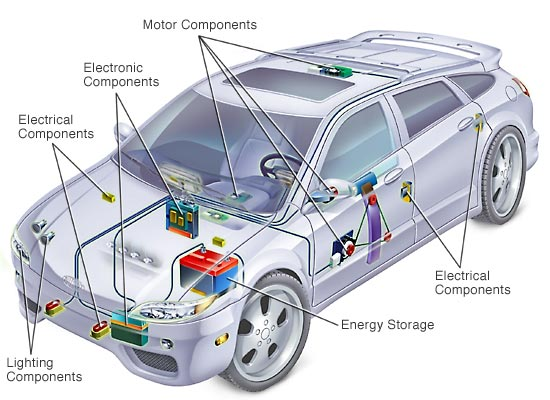
\includegraphics[width=0.5\linewidth]{Figuras/Ch06/fig1.jpg}}
\end{frame}

\begin{frame}{Introdução}
\begin{block}{Dispositivos de comando}
\begin{itemize}
    \item Os dispositivos de comando são todos aqueles que possuem função lógica dentro de um circuito elétrico. 
    \item Esses dispositivos realizam sua \textbf{função lógica }\textbf{permitindo }ou \textbf{bloqueando} a passagem de corrente entre dois ou mais pontos do circuito.
\end{itemize}
\end{block}

\begin{minipage}{0.45\linewidth}
	\centering
	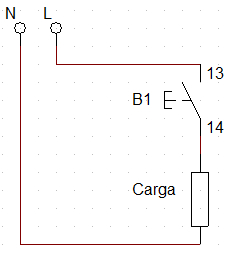
\includegraphics[width=0.6\linewidth]{Figuras/Ch06/fig2.jpg}
	
	Lógica NA
\end{minipage}
\hfill
\begin{minipage}{0.45\linewidth}
	\centering
	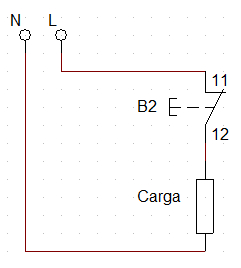
\includegraphics[width=0.6\linewidth]{Figuras/Ch06/fig3.jpg}
	
	Lógica NF
\end{minipage}
\end{frame}

\begin{frame}{Associação de contatos}
\begin{block}{Associações de contatos NA}
\begin{itemize}
    \item Os dispositivos de comando podem ser \textbf{associados} para realizar funções lógicas mais \textbf{complexas}.
    \item Os contatos NA, por exemplo, podem ser associados das seguintes formas:
\end{itemize}
\end{block}

\begin{minipage}{0.45\linewidth}
	\centering
	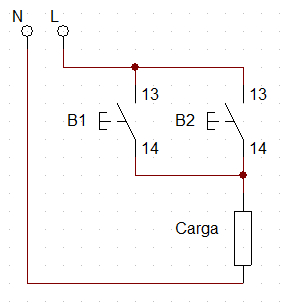
\includegraphics[width=0.7\linewidth]{Figuras/Ch06/fig4.jpg}
	
	Associação NA paralelo
\end{minipage}
\hfill
\begin{minipage}{0.45\linewidth}
	\centering
	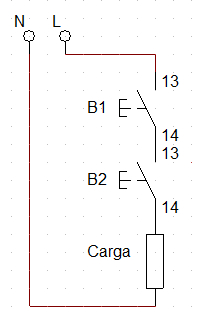
\includegraphics[width=0.5\linewidth]{Figuras/Ch06/fig5.jpg}
	
	Associação NA série
\end{minipage}
\end{frame}

\begin{frame}{Associação de contatos}
\begin{block}{Associações de contatos NA}
\begin{itemize}
    \item Contatos NA associados em \textbf{paralelo} vão ter o efeito conhecido como "ou", isso é, se um deles \textbf{OU} o outro estiver acionado isso equivale à um \textbf{circuito fechado}.
    \item Na eletrônica digital representamos essa relação com o símbolo "$ + $".
\end{itemize}
\end{block}
\end{frame}

\begin{frame}{Associação de contatos}
\begin{block}{Associações de contatos NA}
	O circuito abaixo pode ser escrito como:
	$$ \text{Carga} = \text{B}1+\text{B}2 $$
	
	isso é, a carga será acionada caso B1 \textbf{OU} B2 sejam acionados (ou os dois ao mesmo tempo, claro).
\end{block}

\centerline{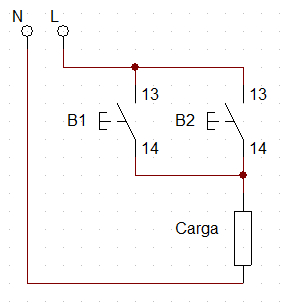
\includegraphics[width=0.35\linewidth]{Figuras/Ch06/fig4.jpg}}
\end{frame}

\newcommand{\nop}{repouso}
\newcommand{\yep}{acionado}

\begin{frame}{Associação de contatos}
\begin{block}{Associações de contatos NA}
	A relação OU também pode ser expressa através de uma \textbf{tabela verdade}, que é útil para entendermos as relações entre os dispositivos de comando e a carga acionada.
	
	Abaixo temos a tabela verdade para a relação:
	$$ \text{Carga} = \text{B}1+\text{B}2 $$
\end{block}

\begin{table}[h]
	\scalebox{1.5}{\begin{tabular}{ccc}
			\toprule
			B1 & B2 & Carga\\ \midrule
			\nop & \nop & \nop \\
			\yep & \nop & \yep \\
			\nop & \yep & \yep \\
			\yep & \yep & \yep \\ \bottomrule
	\end{tabular}}
\end{table}

\end{frame}


\begin{frame}{Associação de contatos}
\begin{block}{Associações de contatos NA}
\begin{itemize}
    \item Contatos NA associados em \textbf{série} vão ter o efeito conhecido como "e", isso é, se um deles \textbf{E} o outro estiverem acionados simultaneamente isso equivale à um \textbf{circuito fechado}.
    \item Na eletrônica digital representamos essa relação com o símbolo "$ \cdot $".
\end{itemize}
\end{block}
\end{frame}

\begin{frame}{Associação de contatos}
\begin{block}{Associações de contatos NA}
	O circuito abaixo pode ser escrito como:
	$$ \text{Carga} = \text{B}1\cdot \text{B}2 $$
	
	 isso é, a carga será acionada caso B1 \textbf{E} B2 sejam acionados simultaneamente.
\end{block}

\centerline{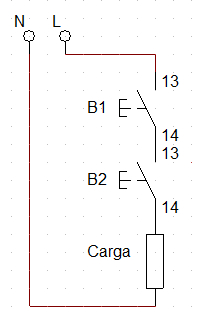
\includegraphics[height=0.5\textheight]{Figuras/Ch06/fig5.jpg}}
\end{frame}

\begin{frame}{Associação de contatos}
\begin{block}{Associações de contatos NA}
	Abaixo temos a tabela verdade para a relação:
	$$ \text{Carga} = \text{B}1\cdot \text{B}2 $$
\end{block}

\vspace{0.3cm}

\begin{table}[h]
	\scalebox{1.5}{\begin{tabular}{ccc}
			\toprule
			B1 & B2 & Carga\\ \midrule
			\nop & \nop & \nop \\
			\yep & \nop & \nop \\
			\nop & \yep & \nop \\
			\yep & \yep & \yep \\ \bottomrule
	\end{tabular}}
\end{table}
\end{frame}


\begin{frame}{Associação de contatos}
\begin{block}{Associações de contatos NF}
\begin{itemize}
    \item Os contatos NF podem ser associados das mesma formas que os contatos NA:
\end{itemize}
\end{block}

\begin{minipage}{0.45\linewidth}
	\centering
	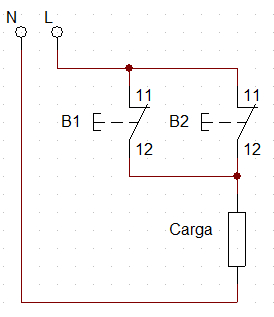
\includegraphics[width=0.7\linewidth]{Figuras/Ch06/fig6.jpg}
	
	Associação NF paralelo
\end{minipage}
\hfill
\begin{minipage}{0.45\linewidth}
	\centering
	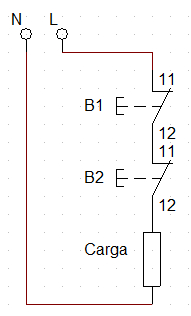
\includegraphics[width=0.5\linewidth]{Figuras/Ch06/fig7.jpg}
	
	Associação NF série
\end{minipage}
\end{frame}


\begin{frame}{Associação de contatos}
\begin{block}{Associações de contatos NF}
\begin{itemize}
    \item As associações de contatos são universais e possuem a mesma simbologia independendo de os contatos serem NA ou NF. Os contatos NF, porém, serão simbolizados de forma diferente, ganhando uma barra em cima do símbolo.
    \item O contato abaixo, por exemplo, pode ser simbolizado por "$ \overline{\text{B}1} $".
\end{itemize}
\end{block}

\vspace{0.2cm}

\begin{center}
	\begin{tikzpicture}[scale=1.5]
	\draw (1.8,0.3) -- +(0.2,0) (1.8,0.3) -- ++(0,0.4) -- +(0.2,0);
	\draw[loosely dashed] (1.8,0.5) -- +(0.85,0);
	\draw (2,0) ++(0.5, 1) -- +(0,0.2) (2,0) ++(0.5,0) -- +(0,-0.2);
	\draw (2,0) ++(0.5,0) -- ++(0.3,1) -- +(-0.3,0);
	\node at (1.5, 0.5) {B1};
	\end{tikzpicture}
\end{center}
\end{frame}

\begin{frame}{Associação de contatos}
\begin{block}{Associações de contatos NF}
O circuito abaixo pode ser escrito como: 
$$ \text{Carga} = \overline{\text{B}1}+\overline{\text{B}2} $$ 

isso é, a carga será acionada caso B1 \textbf{OU} B2 estejam em repouso (ou os dois ao mesmo tempo, claro).
\end{block}

\centerline{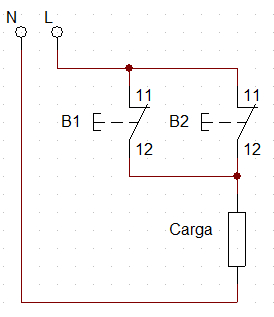
\includegraphics[height=0.5\textheight]{Figuras/Ch06/fig6.jpg}}
\end{frame}

\begin{frame}{Associação de contatos}
\begin{block}{Associações de contatos NF}
Abaixo temos a tabela verdade para a relação:
$$ \text{Carga} = \overline{\text{B}1}+\overline{\text{B}2} $$
\end{block}

\vspace{0.3cm}

\begin{table}[h]
\scalebox{1.5}{\begin{tabular}{ccc}
	\toprule
	B1 & B2 & Carga\\ \midrule
	\nop & \nop & \yep \\
	\yep & \nop & \yep \\
	\nop & \yep & \yep \\
	\yep & \yep & \nop \\ \bottomrule
\end{tabular}}
\end{table}

\end{frame}


\begin{frame}{Associação de contatos}
\begin{block}{Associações de contatos NF}
O circuito abaixo pode ser escrito como:
$$ \text{Carga} = \overline{\text{B}1}\cdot\overline{\text{B}2} $$

isso é, a carga será acionada caso B1 \textbf{E} B2 estejam em repouso simultaneamente.
\end{block}

\centerline{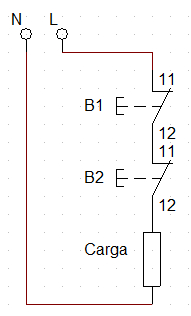
\includegraphics[height=0.5\textheight]{Figuras/Ch06/fig7.jpg}}
\end{frame}

\begin{frame}{Associação de contatos}
\begin{block}{Associações de contatos NF}
Abaixo temos a tabela verdade para a relação:
$$ \text{Carga} = \overline{\text{B}1}\cdot\overline{\text{B}2} $$
\end{block}

\vspace{0.3cm}

\begin{table}[h]
\scalebox{1.5}{\begin{tabular}{ccc}
\toprule
B1 & B2 & Carga\\ \midrule
\nop & \nop & \yep \\
\yep & \nop & \nop \\
\nop & \yep & \nop \\
\yep & \yep & \nop \\ \bottomrule
\end{tabular}}
\end{table}
\end{frame}


\begin{frame}{Elementos do circuito de comando}
\begin{block}{Principais elementos}
	Os principais elementos estudados em comandos elétricos são:
	\begin{itemize}
		\item Botões (botoeiras)
		\item Contatores
		\item Relés
		\item Temporizadores
	\end{itemize}
	Todos eles possuem função lógica, podendo ser eles próprios ou suas chaves associados como vimos anteriormente.
\end{block}
\end{frame}


\begin{frame}{Elementos do circuito de comando}
\begin{block}{Botões (botoeiras)}
	Os botões já foram discutidos anteriormente, mas vale citar:
	\begin{itemize}
		\item A botoeira é um \textit{elemento de sinal}, isto é, deve ser usada somente no circuito de comando para enviar sinais à outros componentes.
		\item Na indústria usamos o nome "botoeira", pois esta possui retorno por mola. Isso é essencial para o funcionamento lógico adequado deste elemento. 
	\end{itemize}
\end{block}
\end{frame}


\begin{frame}{Elementos do circuito de comando}
\begin{block}{Contatores}
	Os contatores também já foram abordados anteriormente, mas vale a pena mencionar seu princípio de funcionamento:
	\begin{itemize}
		\item A parte em cinza consiste em um núcleo magnético fragmentado em duas partes, um delas sendo móvel.
	\end{itemize}
\end{block}

\centerline{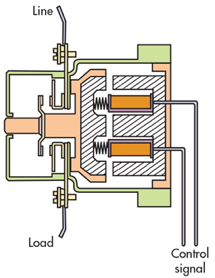
\includegraphics[width=0.3\linewidth]{Figuras/Ch06/fig8.jpg}}
\end{frame}

\begin{frame}{Elementos do circuito de comando}
\begin{block}{Contatores}
	\begin{itemize}
		\item Quando as bobinas (em laranja) são percorridas por corrente geram um fluxo magnético que junta as duas partes magnéticas, movimentando consigo os contatos do componente, que podem se abrir (NF) ou fechar (NA).
	\end{itemize}
\end{block}

\begin{minipage}{0.45\linewidth}
	\centering
	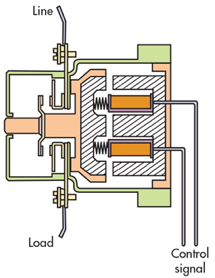
\includegraphics[width=0.6\linewidth]{Figuras/Ch06/fig8.jpg}
	
	Contator desenergizado
\end{minipage}\tikzmark{C1}
\hfill
\begin{minipage}{0.45\linewidth}
	\centering
	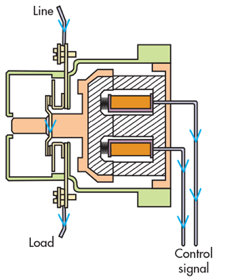
\includegraphics[width=0.6\linewidth]{Figuras/Ch06/fig9.jpg}
	
	Contator energizado
\end{minipage}

\begin{tikzpicture}[overlay, remember picture]
	\draw[-{Latex[length=4mm,width=5mm]}, line width=1.5mm] (C1) -- +(1,0);
\end{tikzpicture}

\end{frame}

\begin{frame}{Elementos do circuito de comando}
\begin{block}{Contatores}
	\begin{itemize}
		\item Quando o fluxo de corrente cessa os núcleos magnéticos são separados por molas.
	\end{itemize}
\end{block}
\begin{minipage}{0.45\linewidth}
	\centering
	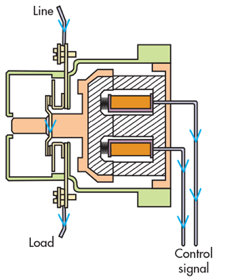
\includegraphics[width=0.6\linewidth]{Figuras/Ch06/fig9.jpg}
	
	Contator energizado
\end{minipage}\tikzmark{C1}
\hfill
\begin{minipage}{0.45\linewidth}
	\centering
	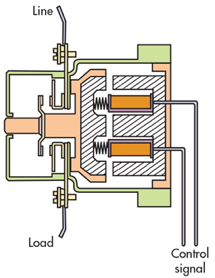
\includegraphics[width=0.6\linewidth]{Figuras/Ch06/fig8.jpg}
	
	Contator desenergizado
\end{minipage}

\begin{tikzpicture}[overlay, remember picture]
\draw[-{Latex[length=4mm,width=5mm]}, line width=1.5mm] (C1) -- +(1,0);
\end{tikzpicture}

\end{frame}

\begin{frame}{Elementos do circuito de comando}
	\centerline{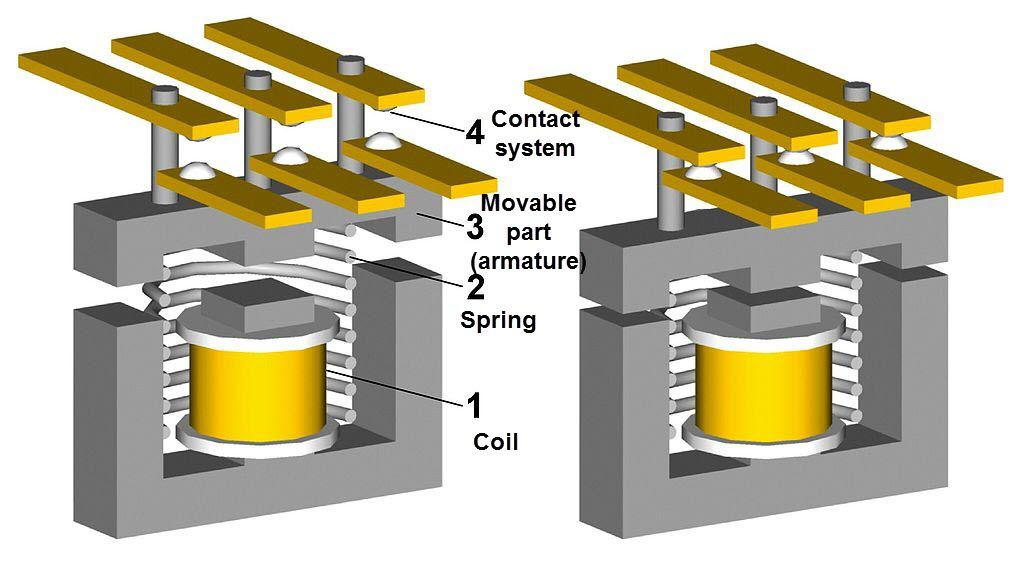
\includegraphics[width=1\linewidth]{Figuras/Ch06/fig10.jpg}}
\end{frame}


\begin{frame}{Elementos do circuito de comando}
\begin{block}{Relés}
\begin{itemize}
    \item Os relés são elementos muito similares aos contatores, porém possuem \textbf{capacidade reduzida}.
    \item Na imagem abaixo podemos notar que os componentes estruturais presentes no relé são muito similares aos do contator. Não há, porém, um núcleo magnético móvel, as únicas coisas que se movem são os \textbf{contatos}.
\end{itemize}
\end{block}
\centerline{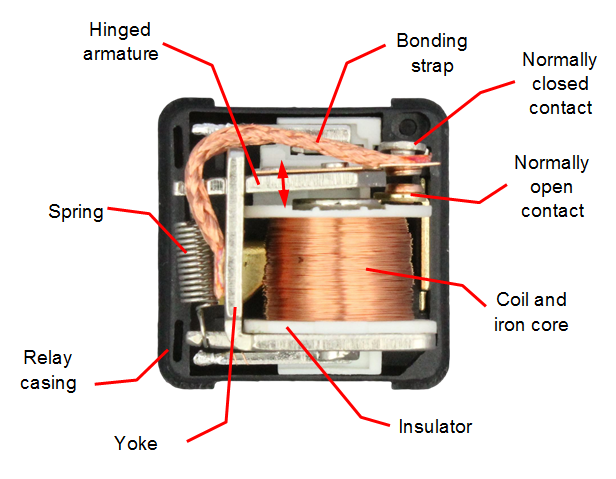
\includegraphics[width=0.45\linewidth]{Figuras/Ch06/fig11.png}}
\end{frame}


\begin{frame}{Elementos do circuito de comando}
\begin{block}{Relés}
\begin{itemize}
    \item Uma aplicação mais interessante dos relés é a proteção do equipamento de potência no circuito de força. Essa proteção é feita pelos chamados \textit{relés térmicos}, que também já foram abordados.
\end{itemize}
\end{block}
\centerline{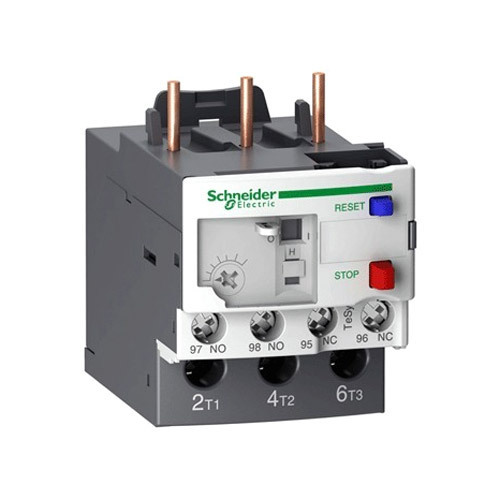
\includegraphics[width=0.5\linewidth]{Figuras/Ch06/fig12.jpg}}
\end{frame}


\begin{frame}{Elementos do circuito de comando}
\begin{block}{Relés}
\begin{itemize}
    \item Outra possível aplicação dos relés é a \textbf{temporização}. Relés com essa função são chamados de relés \textit{de tempo} ou \textit{temporizadores}.
    \item A simbologia dos relés temporizadores e seus contatos é apresentada abaixo.
\end{itemize}
\end{block}
\smallskip
\centerline{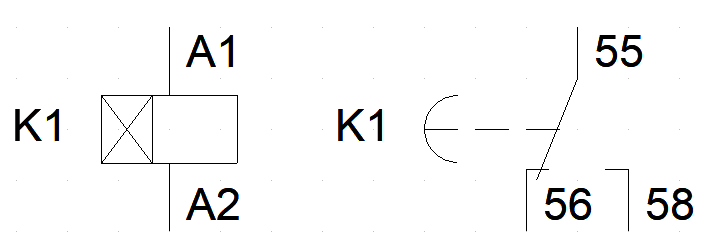
\includegraphics[width=0.8\linewidth]{Figuras/Ch06/fig13.jpg}}
\end{frame}


\begin{frame}{Elementos do circuito de comando}
\begin{block}{Relés}
	\begin{itemize}
		\item Repare que os contatos do relé temporizador são representados por uma chave com \textbf{duas} posições.
		\item Quando o relé está em repouso, os terminais 55-56 estão ligados e quando o relé está acionado os terminais 55-58 se ligam.
	\end{itemize}
\end{block}
\centerline{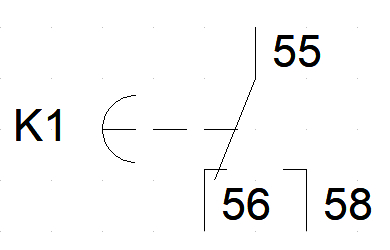
\includegraphics[width=0.6\linewidth]{Figuras/Ch06/fig14.jpg}}
\end{frame}


\begin{frame}{Elementos do circuito de comando}
\begin{minipage}{0.45\linewidth}
	\centering
	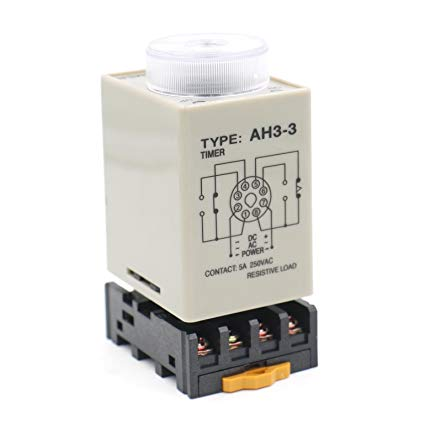
\includegraphics[width=1.3\linewidth]{Figuras/Ch06/fig15.jpg}
\end{minipage}
\hfill
\begin{minipage}{0.45\linewidth}
	\centering
	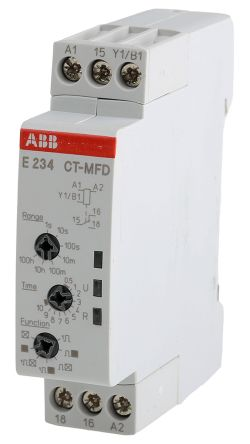
\includegraphics[width=0.6\linewidth]{Figuras/Ch06/fig16.jpg}
\end{minipage}
\end{frame}


\begin{frame}{Elementos do circuito de comando}
\begin{block}{Simbologia}
	\begin{itemize}
		\item Segue abaixo uma tabela apresentando os símbolos literais de acordo com a NBR 5280.
	\end{itemize}
	 \textbf{Nota:} É comum a utilização de "B"~para designar botão.
\end{block}
\begin{table}[h]
	\scalebox{1}{\begin{tabular}{cl}
			\toprule
			Símbolo & \multicolumn{1}{c}{Componente}\\\midrule
			F & Dispositivos de proteção \\
			H & Dispositivos de sinalização \\
			K & Contatores \\
			M & Motores\\
			\multirow{2}{*}{Q} & Dispositivos de manobra \\
			 & para circuitos de potência \\
			\multirow{2}{*}{S} & Dispositivos de manobra e \\
			 & seletores auxiliares \\
			T & Transformadores \\
			\bottomrule
	\end{tabular}}
\end{table}
\end{frame}


\begin{frame}{Elementos do circuito de comando}
\begin{block}{Simbologia}
	A numeração dos contatos que representam terminais de força é feita da seguinte maneira:
	\begin{itemize}
		\item Entrada (linha): 1, 3 e 5
		\item Saída (terminal): 2, 4 e 6
	\end{itemize}
	Já a numeração dos contatos auxiliares segue o seguinte padrão:
	\begin{itemize}
		\item Contato NF: 1 (entrada) e 2 (saída)
		\item Contato NA: 3 (entrada) e 4 (saída)
	\end{itemize}
	Os terminais da bobina de relés e contatores são designados por A1 e A2. Os contatos auxiliares de um contator seguem uma numeração com dois dígito, sendo:
	\begin{itemize}
		\item 1o dígito: indica o número do contato (1, 2, 3...)
		\item 2o dígito: indica o tipo do contato (NA ou NF)
	\end{itemize}
\end{block}
\end{frame}


\frame{
	\frametitle{Exercícios}
	\begin{block}{}
		01. Dar exemplos da utilização de relés temporizadores.
		
		\vspace{0.5cm}
		
		02. Desenhar e fazer a tabela verdade do circuito expresso por: \[ \text{Carga}=\overline{\text{B}1}+\text{B}2 \]
	\end{block}
}

\section*{Referências}
\frame{
	\frametitle{Referências e Exercícios Complementares}
	\begin{itemize}
		\item FILHO, João Mamede. Instalações Elétricas Industriais, 6 ed. Rio de Janeiro, LTC, 2001.
	\end{itemize}
	%\centering{\alert{Página 546 - \textbf{Capítulo 6}}} \\
	%\centering{\alert{Lista de exercícios 01}}
}
